% file: elektroskop.tex
\documentclass[tikz,border=5pt]{standalone} % standalone für einzelne Abbildungen
\usepackage{tikz}

\begin{document}

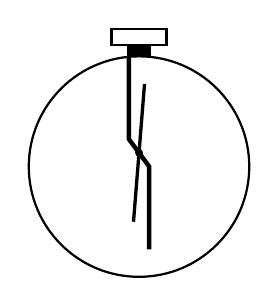
\begin{tikzpicture}[scale=0.7]
    % -- Gehäuse (Kreis) --
    \draw[thick] (0,2) circle (2);

    % -- Isolator (kleiner Block) --
    \filldraw[thick] (-0.2,4) rectangle (0.2, 4.2);

    % -- Metallplatte oben --
    \draw[thick] (-0.5,4.2) rectangle (0.5, 4.5);

    % -- Eckiges S-Gestell --
    \draw[ultra thick]
        (-0.185,4)
        -- (-0.185,2.5)
        -- (0.185,2.0)
        -- (0.185,0.5);

    % -- Zeiger (am unteren Ende des S-Gestells) --
    \draw[very thick] (0.1,3.5) -- (-0.1,1);
    \filldraw[thick] (0, 2.25) circle (0.05);
\end{tikzpicture}

\end{document}
